\chapter{Cryptographic Preliminaries}

This chapter provides some cryptographic background information which is
relevant for the attribute-based credential systems which we describe in the
next chapters. In particular we focus on public-key cryptography in which a key
consists of a public and a private part. These key pairs are constructed such
that deriving the private part of the key from the public part is equivalent to
solving a computational problem that is considered extremely difficult.

\section{RSA Cryptography}\index{RSA}

In an RSA-based cryptosystem~\cite{RSA1978} a key pair consists of a public part
$(n, e)$ and a private part $d$. The RSA modulus $n = p \cdot q$ is the product
of two primes $p$ and $q$ and the public exponent $e$ is a value that satisfies
$1 < e < \phi(n)$ and $gcd(e, \phi(n)) = 1$ where $\phi(n) = (p-1)(q-1)$ is
Euler's totient function\footnote{Euler's totient function $\phi(n)$ computes
the number of positive integers less then or equal to $n$ that are relatively
prime to $n$. An integer $k$ is relatively prime to $n$ if $gcd(k, n) = 1$.}.
The private exponent $d$ is a value that satisfies $1 < d < \phi(n)$ and
$e \cdot d = 1 \mod \phi(n)$, hence it can be computed as
$d = e^{-1} \mod \phi(n)$. When $p$ and $q$ are know, this computation is easy,
but computing $d$ based on just $n$ and $e$ is proved to be computationally
equivalent to determining the prime factors $p$ and $q$ of $n$, which is known
as the integer factorisation problem, a number-theoretic problem which is
considered intractable for large integers.

\subsection{Encryption Scheme}\index{RSA!encryption}

Such an RSA key pair can then be used to encrypt a message $m$ into an RSA
ciphertext $c = m^e \mod n$ using Algorithm~\ref{alg:RSA-encrypt}. Decryption
of such a ciphertext using Algorithm~\ref{alg:RSA-decrypt} is based on the fact
that
\begin{equation*}
  c^d = (m^e)^d = m^{e \cdot d} = m \mod n\text.
\end{equation*}

\begin{algorithm}[ht]
  \caption{Basic RSA encryption.}
  \label{alg:RSA-encrypt}
  \addtolength{\baselineskip}{1mm}
  \begin{algorithmic}[1]
    \Function{RSA-encrypt}{$(n, e), m$}
      \State $c \gets m^e \mod n$
      \Return $c$
    \EndFunction
  \end{algorithmic}
\end{algorithm}
\begin{algorithm}[ht]
  \caption{Basic RSA decryption.}
  \label{alg:RSA-decrypt}
  \addtolength{\baselineskip}{1mm}
  \begin{algorithmic}[1]
    \Function{RSA-decrypt}{$(n, e), c, d$}
      \State $m \gets c^d \mod n$
      \Return $m$
    \EndFunction
  \end{algorithmic}
\end{algorithm}

The problem of recovering the message $m$ based on the ciphertext $m^e \mod n$
and public key $(n, e)$ is known as the \emph{RSA problem}\index{RSA problem}.
This is equivalent to finding $e$th roots modulo $n$ which is assumed to be as
difficult as the integer factorisation problem\index{integer factorisation
problem}. Hence, the \emph{RSA assumption}\index{RSA assumption} states that
the probability that an attacker can solve the RSA problem is negligible.

Note that the algorithms described in this thesis are the basic textbook
versions, which are vulnerable to a range of attacks~\cite{Hastad1985,
Coppersmith1997}. To prevent such attacks, practical RSA implementations
typically include some form of randomized padding into the value $m$ before
encrypting it. For example, for encryption one would normally use the OAEP
padding scheme from the PKCS \#1 standard~\cite{PKCS_1}. The same holds for RSA
signatures, as described below, where usually the PSS padding
scheme~\cite{PKCS_1} is used to securely pad messages before signature
generation.

\subsection{Signature Schemes}

In a similar fashion, this construction can also be used to create digital
signatures. To generate an RSA signature with Algorithm~\ref{alg:RSA-sign}, the
signer computes the message digest $h = \Call{Hash}{m}$ of the message to be
signed $m$ using a cryptographic hash function $\Call{Hash}{}$. This $h$, which
serves as a fingerprint of the original message, is then raised to the private
exponent. The result of this operation is the signature $s = h^d \mod n$ over
the message $m$.\index{RSA!signature}
Such an RSA signature can be verified using Algorithm~\ref{alg:RSA-verify}. The
verifier recovers the fingerprint $\hat{h} = s^e \mod n$ from the signature
value $s$ using the public exponent $e$ and checks whether this matches with the
message digest of the message $m$. If they match, the signature is valid,
otherwise the signature is invalid. The security of this RSA signature scheme is
also based on the RSA assumption.

\begin{algorithm}[H]
  \caption{Basic RSA signature generation.}
  \label{alg:RSA-sign}
  \addtolength{\baselineskip}{1mm}
  \begin{algorithmic}[1]
    \Function{RSA-sign}{$(n, e), m, d$}
      \State $h \gets \Call{Hash}{m}$
      \State $s \gets h^d \mod n$
      \Return $s$
    \EndFunction
  \end{algorithmic}
\end{algorithm}
\begin{algorithm}[H]
  \caption{Basic RSA signature verification.}
  \label{alg:RSA-verify}
  \addtolength{\baselineskip}{1mm}
  \begin{algorithmic}[1]
    \Function{RSA-verify}{$(n, e), m, s$}
      \State $\hat{h} \gets s^e \mod n$
      \If{$\hat{h} \neq \Call{Hash}{m}$}
        \Return \Call{Invalid}{}
      \EndIf
      \Return \Call{Valid}{}
    \EndFunction
  \end{algorithmic}
\end{algorithm}

Some other signature schemes based on the RSA cryptosystem, such as the
Camenisch-Lysyanskaya scheme~\cite{CamenischLysyanskaya2003}
\index{Camenisch-Lysyanskaya scheme} which is described
in Section~\ref{sec:CL-scheme}, only use the RSA modulus\index{RSA modulus} $n$ as the public part
of the key, whereas the private part consists of the primes $p$ and $q$. This
allows them to generate a fresh exponent $e$ for each signature which will then
become part of the signature. Since an attacker can now control both the
signature and the exponent, solving the RSA problem has become easier. Hence a
stronger assumption is needed. This \emph{strong RSA assumption}\index{strong RSA assumption} states that the
probability that an attacker can solve the RSA problem is negligible, even when
the attacker can chose the public exponent $e$.

\section{Discrete Logarithm Cryptography}

In a discrete logarithm-based cryptosystem~\cite{DH1976,ElGamal1985} a key pair
is accompanied with a description of the prime-order group in which the
computations take place. As an example we use $(p, q, g)$, where $p$ is a prime,
$q$ is a prime divisor of $p-1$, and $g$ is a generator, with order $q$, of a
subgroup of $\Z^*_p$. A private part of the key in such system is a random value
$x$ and the corresponding public part is $h = g^x \mod p$. The problem of
computing the private part $x = \log_g h$, based on the description of the group
$(p, q, g)$ and the public part $h$, is known as the \emph{discrete logarithm
problem}\index{discrete logarithm problem}.

\subsection{Key Agreement Scheme}\index{Diffie-Hellman key agreement}

The first discrete logarithm-based scheme was the key agreement scheme by Diffie
and Hellman~\cite{DH1976}. In this scheme a key pair as described above can be
used to compute a shared key with another party that uses the same group
parameters. To this end, both parties generate such a key pair and send their
public key to each other. Next, they compute the modular exponentiation of the
received value and their private key, as depicted in Figure~\ref{msc:DH}. The
result of this computation can then be used as a shared key\index{shared key}
since
\begin{equation*}
  h_2^{x_1} = (g^{x_2})^{x_1} = g^{x_2 \cdot x_1}
  = k = g^{x_1 \cdot x_2} = (g^{x_1})^{x_2} = h_1^{x_2} \mod p
\end{equation*}
The problem of computing $k$, based on both public keys $h_1$ and $h_2$ and the
group description $(p, q, g)$, is assumed to be as difficult as the discrete
logarithm problem and is called the \emph{(computational) Diffie-Hellman problem}\index{Diffie-Hellman problem}. A related
problem is to determine whether a value $y$ is created using $h_1$ and $h_2$,
hence whether $y = g^{x_1 \cdot x_2}$, or not. This is known as the
\emph{decisional Diffie-Hellman problem}\index{decisional Diffie-Hellman
problem}.

\begin{figure}[ht]
  \centering
  \includegraphics[scale=.45]{mscs/dh}
  \caption{Diffie-Hellman key agreement protocol.}
  \label{msc:DH}
\end{figure}

\subsection{Encryption}

The first encryption scheme based on discrete logarithms was proposed by
ElGamal~\cite{ElGamal1985}. In order to encrypt a message $m$, the user
generates a random value $r$ and commits to it by computing $c_1 = g^r \mod p$.
The value $r$ is then used to randomise the public key which is multiplied with
the message to obtain the encrypted message $c_2 = m \cdot h^r \mod p$. The
resulting ciphertext consists of both $c_1$ and $c_2$ (see Algorithm~\ref{alg:ElGamal-encrypt}).
In contrast to the RSA encryption scheme, the ElGamal encryption algorithm
produces a different ciphertext each time although the inputs remain the same.

The message $m$ can be recovered from a ciphertext $(c_1, c_2)$ by dividing
$c_2$ by $c_1^x = g^{r \cdot x} = h^r \mod p$, as described in Algorithm~\ref{alg:ElGamal-decrypt}. An attacker, who does not have
the private key $x$, must determine $h^r = g^{x \cdot r} \mod p$ based on the
public key $h = g^x \mod p$ and the commitment $c_1 = g^r \mod p$, that is, he
must solve the Diffie-Hellman problem.

\begin{algorithm}[ht]
  \caption{ElGamal encryption.}
  \label{alg:ElGamal-encrypt}
  \addtolength{\baselineskip}{1mm}
  \begin{algorithmic}[1]
    \Function{ElGamal-encrypt}{$(p, q, g), h, m$}
      \State $r \gets \Call{Random}{}$
      \State $c_1 \gets g^r \mod p$
      \State $c_2 \gets m \cdot h^r \mod p$
      \Return $(c_1, c_2)$
    \EndFunction
  \end{algorithmic}
\end{algorithm}
\begin{algorithm}[ht]
  \caption{ElGamal decryption.}
  \label{alg:ElGamal-decrypt}
  \addtolength{\baselineskip}{1mm}
  \begin{algorithmic}[1]
    \Function{ElGamal-decrypt}{$(p, q, g), (c_1, c_2), x$}
      \State $m \gets c_2 \cdot c_1^{-x} \mod p$
      \Return $m$
    \EndFunction
  \end{algorithmic}
\end{algorithm}

\subsection{Signatures}

Many signature schemes have been based on the discrete logarithm problem, for
example the Chaum-Pedersen scheme which is described in
Section~\ref{sec:CP-scheme}, but also the ElGamal signature scheme~\cite{ElGamal1985}
of which a variant, known as the Digital Signature Algorithm, is part of the
Digital Signature Standard of the United States government.
Like ElGamal's encryption scheme, the signature $(s_1, s_2)$ consists of two
parts generated using Algorithm~\ref{alg:ElGamal-sign}. The first is a
commitment to the randomisation value $r$, whereas the second part commits to
the fingerprint $c$ of the message $m$ that is to be signed. In the unlikely
case that the resulting $s_2$ is 0, these steps have to be repeated to obtain a
usable signature.

This signature can be verified using Algorithm~\ref{alg:ElGamal-verify}. We
cannot recover the message fingerprint from the signature, as was the case
with RSA, but we can check it according to the following equation:
\begin{equation*}
  h^{s_1} \cdot s_1^{s_2}
  = g^{x \cdot s_1} \cdot g^{r \cdot s_2}
  = g^{x \cdot s_1} \cdot g^{r \cdot r^{-1} \cdot (c - x \cdot s_1)}
  = g^{x \cdot s_1} \cdot g^{c - x \cdot s_1}
  = g^c \mod p
\end{equation*}

\begin{algorithm}
  \caption{ElGamal signature generation.}
  \label{alg:ElGamal-sign}
  \addtolength{\baselineskip}{1mm}
  \begin{algorithmic}[1]
    \Function{ElGamal-sign}{$(p, q, g), m, x$}
      \State $c \gets \Call{Hash}{m}$
      \State $r \gets \Call{Random}{~}$
      \State $s_1 \gets g^r \mod p$
      \State $s_2 \gets r^{-1} \cdot (c - x \cdot s_1) \mod (p - 1)$
      \Return $(s_1, s_2)$
    \EndFunction
  \end{algorithmic}
\end{algorithm}
\begin{algorithm}
  \caption{ElGamal signature verification.}
  \label{alg:ElGamal-verify}
  \addtolength{\baselineskip}{1mm}
  \begin{algorithmic}[1]
    \Function{ElGamal-verify}{$(p, q, g), m, (s_1, s_2), h$}
      \State $c \gets \Call{Hash}{m}$
      \If{$h^{s_1} \cdot s_1^{s_2} \neq g^c \mod p$}
        \Return \Call{Invalid}{}
      \EndIf
      \Return \Call{Valid}{}
    \EndFunction
  \end{algorithmic}
\end{algorithm}

\section{Elliptic Curve Cryptography}

In the previous section we described the discrete logarithm cryptography in a
setting of a prime order subgroup of $\Z^*_p$. These techniques can, however,
be applied to any finite cyclic group. Another popular setting for implementing
discrete logarithm systems is the elliptic curve setting which we describe below.

Note that it is common to use additive notation in an elliptic curve setting,
whereas multiplicative notation is typically used to denote operations in prime
order subgroups.

\subsection{Elliptic Curves}

A finite field containing $q$ elements, where $q = p^k$ is a prime power, is
denoted as $\F{q}$. An example of such a field is $\Z_p$, but more complex
finite fields can also be used for elliptic curves. An elliptic curve $E$ over
$\F{q}$ is defined by the equation
\begin{equation}\label{eqn:elliptic_curve}
  E: y^2 = x^3 + a \cdot x + b
\end{equation}
where $a, b \in \F{q}$ are the curve parameters that satisfy
$4 \cdot a^3 + 27 \cdot b^2 \neq 0$. This condition is required for E to be
non-singular, as required for cryptographic applications. The set of all points
$P = (x, y)$ on this curve $E$ is denoted as
\begin{equation*}
  E(\F{q}) = \{ (x, y) \in \F{q} \times \F{q} : y^2 = x^3 + a \cdot x + b \}
                         \cup \{ \infty \}
\end{equation*}
where $\infty$ is a special point called the \emph{point at infinity}.


\begin{figure}[ht]
  \centering
  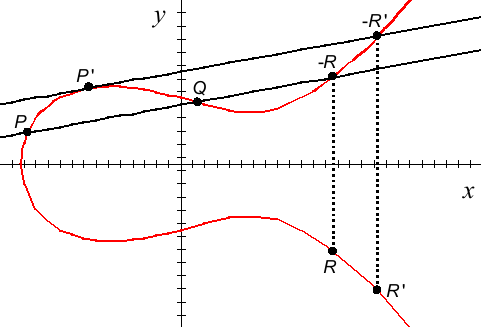
\includegraphics[scale=.5]{images/ec_math}
  \caption[Geometric visualisation of point operations on an elliptic curve.]{
    Geometric visualisation of point addition ($R = P + Q$), point doubling
    ($R' = 2P'$) and point negation ($-R$) on an elliptic curve.}
  \label{fig:EC}
\end{figure}

On these points three basic operations can be defined: negation, addition and
doubling. These operations are detailed below and visualised geometrically in
Figure~\ref{fig:EC}.
\begin{enumerate}
  \item \emph{Point negation}, the \emph{negative} $R = -P$, of the point $P$
    is computed according to Algorithm~\ref{alg:ec_point_negation}.
    Geometrically, this is the reflection of point $P$ in the $x$-axis.
    \begin{algorithm}[H]
      \caption{Elliptic curve point negation: $R = -P$}
      \label{alg:ec_point_negation}

      \begin{algorithmic}[1]
        \Function{ECPointNegation}{$P$}
          \If{$P = \infty$}
            \Return $\infty$
          \EndIf

          \State $(x_P, y_P) \gets P$

          \Return $(x_P, -y_P)$
        \EndFunction
      \end{algorithmic}
    \end{algorithm}

  \item \emph{Point addition}, the \emph{sum} $R = P + Q$, of the points $P$
    and $Q$ is computed using Algorithm~\ref{alg:ec_point_addition}.
    In geometry, this is the reflection in the $x$-axis of the intersection of
    the curve and the line through the points $P$ and $Q$.
    \begin{algorithm}[H]
      \caption{Elliptic curve point addition: $R = P + Q$}
      \label{alg:ec_point_addition}

      \begin{algorithmic}[1]
        \Function{ECPointAddition}{$P$, $Q$}
          \If{$P = \infty$}
            \Return $Q$
          \EndIf
          \If{$P = Q$}
            \Return $2 \cdot P$
          \EndIf
          \If{$P = -Q$ or $Q = \infty$}
            \Return $\infty$
          \EndIf

          \State $(x_P, y_P) \gets P$
          \State $(x_Q, y_Q) \gets Q$

          \State $x \gets \left(\dfrac{y_Q - y_P}{x_Q - x_P}\right)^2 - x_P - x_Q \mod q$
          \State $y \gets \left(\dfrac{y_Q - y_P}{x_Q - x_P}\right) (x_P - x_R) - y_P \mod q$

          \Return $(x, y)$
        \EndFunction
      \end{algorithmic}
    \end{algorithm}

  \item \emph{Point doubling}, the \emph{double} $R = 2 \cdot P$ is computed
    using Algorithm~\ref{alg:ec_point_doubling}. Geometrically, this is the
    reflection in the $x$-axis of the intersection of the curve and the tangent
    line to the curve at the point $P$, see Figure~\ref{fig:EC}.
    \begin{algorithm}
      \caption{Elliptic curve point doubling: $R = 2 \cdot P$}
      \label{alg:ec_point_doubling}

      \begin{algorithmic}[1]
        \Function{ECPointDoubling}{$P$}
          \If{$P = \infty$}
            \Return $P$
          \EndIf

          \State $(x_P, y_P) \gets P$

          \State $x_R \gets \left(\dfrac{3 x_P^3 + a}{2 y_P}\right)^2 - 2 x_P \mod q$
          \State $y_R \gets \left(\dfrac{3 x_P^3 + a}{2 y_P}\right) (x_P - x_R) - y_P \mod q$

          \Return $(x_R, y_R)$
        \EndFunction
      \end{algorithmic}
    \end{algorithm}
\end{enumerate}

Furthermore, based on these basic operations we can define \emph{point
multiplication} as the multiplication of a point $P$ with an integer $k$, which
is denoted as $k \cdot P$. To compute this multiplication various methods exist.
A basic solution is the repeated-double-and-add method given in
Algorithm~\ref{alg:ec_point_multiplication}. The inverse of this operation is to
find an integer $k$ such that $Q = k \cdot P$ for given points $P$ and $Q$. This
is a hard problem which is know as the \emph{elliptic curve discrete logarithm
problem}.

\begin{algorithm}
  \caption{Elliptic curve point multiplication: $R = k \cdot P$}%(repeated-double-and-add; right-to-left binary method)
  \label{alg:ec_point_multiplication}

  \begin{algorithmic}[1]
    \Function{ECPointMultiplication}{$k$, $P$}
      \State $(k_{l-1}, \dots, k_1, k_0) \gets k$ \Comment{binary representation of $k$}
      \State $R \gets \infty$

      \For{$i$ from $0$ to $l - 1$}
        \If{$k_i = 1$}
          \State $R \gets R + P$
        \EndIf
        \State $P \gets 2P$
      \EndFor

      \Return $R$
    \EndFunction
  \end{algorithmic}
\end{algorithm}

Finally, if we know the $x$-coordinate of a point on the curve, the square of
the corresponding $y$-coordinate is known, namely as defined in
(\ref{eqn:elliptic_curve}). By taking the square root of $x^{3} + a \cdot x + b$ we
find either $y$ or $-y$. This method of \emph{point reconstruction} forms the
basis of \emph{point compression}, for compact representation of points.

The points on the elliptic curve $E$ form a finite cyclic group with point
addition as the group operation and the point at infinity as the zero-element.
Hence, such a group can be used to implement discrete logarithm-based
cryptography. An example to show how easy it is to translate the algorithms and
protocols for discrete logarithm-based cryptography to the elliptic curve
setting is given in Figure~\ref{msc:ECDH}. Like its counterpart from
Figure~\ref{msc:DH}, this version of the Diffie-Hellman key agreement protocol
also computes a shared key $K = x_1 \cdot x_2 \cdot P$. The only difference is
that $K$ is now a point instead of an integer.

\begin{figure}[ht]
  \centering
  \includegraphics[scale=.45]{mscs/ecdh}
  \caption{Elliptic curve version of the Diffie-Hellman key agreement protocol.}
  \label{msc:ECDH}
\end{figure}

\subsection{Pairings\label{sec:pairings}}

Besides an alternative implementation for discrete logarithm-based cryptography,
elliptic curves also offer additional functionality, such as efficiently
computable bilinear pairings.

A bilinear pairing is a map of the form $e: \mathbb{G}_1 \times \mathbb{G}_2 \to
\mathbb{G}_T$ where $\mathbb{G}_1$ and $\mathbb{G}_2$ are typically additive
groups and $\mathbb G_T$ is a multiplicative group. Bilinearity means that the
map is linear in both components. This bilinearity property can be written as
follows:
\begin{equation*}
  \begin{array}{rcl}
    e(P + P',\; Q) & = & e(P,\; Q)\cdot e(P',\; Q) \\
     & \text{and} & \\
    e(P,\; Q + Q') & = & e(P,\; Q)\cdot e(P,\; Q')
  \end{array}
\end{equation*}
As a result, $e(n\cdot P,\; m\cdot Q) = e(P,\; Q)^{n \cdot m}$.

Pairings are used for many (new) cryptographic protocols~\cite{BSS05}, such as
short signatures~\cite{BonehLS04}, three-party one-round key
agreement~\cite{Joux04}, identity based encryption~\cite{BonehFranklin01} and
anonymous credentials~\cite{CamenischLysyanskaya04}. There are different
pairings that can be used for this kind of cryptography, for example the Weil
pairing, Tate pairing, ate pairing and the recent R-ate pairing~\cite{Vercauteren09}.
For all these pairings one often uses specific cyclic subgroups of a curve
$E(\mathbb{F}_{p^k})$ as $\mathbb{G}_1$ and $\mathbb{G}_2$ and
$\mathbb{F}_{p^k}^*$ as $\mathbb{G}_T$.

\subsubsection{Barreto-Naehrig Curves\label{sec:BN}}\index{Barreto-Naehrig curves}

Pairing-friendly elliptic curves are curves with a small embedding degree and a
large prime-order subgroup~\cite{FreemanST2010}. In 2005, Barreto and Naehrig
discovered a new method
for constructing pairing friendly elliptic curves of prime order over a prime
field~\cite{BN06}. More precisely, Barreto-Naehrig curves are defined over
$\F{p}$ where $p = p(u) = 36 u^4 + 36 u^3 + 24 u^2 + 6 u + 1$ for $u \in \Z$
such that $p$ is prime. The order of such curve is a prime $n$ where
$n = n(u) = 36 u^4 + 36 u^3 + 18 u^2 + 6 u + 1$. Hence, a Barreto-Naehrig curve
is constructed by generating integers $u$ until both $p(u)$ and $n(u)$ are prime
numbers.

\section{Proofs of Knowledge}

A cryptographic concept that is frequently used in attribute-based credential is
a \emph{proof of knowledge}\index{proof of knowledge}. The goal of such proof is for the user, or
\emph{prover}, to convince the verifier of a given statement. For example, the
often used challenge-response construction in which a user has to sign or
decrypt a challenge to authenticate herself, is a proof that she knows the
private key corresponding to the public key used by the verifier.

To describe such proofs of knowledge we use the notation introduced by Camenisch
and Stadler~\cite{CamenischStadler1997}. For example,
\begin{equation*}
  PK\{(\alpha) : h = g^{\alpha} \mod p \}
\end{equation*}
denotes a proof of knowledge of a value $\alpha$ such that $h = g^{\alpha} \mod p$,
that is, a proof of knowledge of the private part of a discrete logarithm key
pair.

\subsection{Zero-knowledge Protocols}

In this section we describe zero-knowledge protocols as a way to convince a
verifier. The protocols have the property that no matter what a verifier does,
he will not be able to extract any useful information from the user. More
precisely, the term \emph{zero-knowledge} refers to the fact that whatever
information the verifier learns from the user, that information could have been
generated by the verifier on its own, without the assistance of the user.
However, a verifier that actually carried out the protocol will be convinced
that the user has the specified knowledge, in our example, the private key.

A well-known example of a zero-knowledge protocol is Schnorr's identification
protocol~\cite{Schnorr1991}, which proves knowledge of a discrete logarithm.
This protocol is depicted in Figure~\ref{msc:schnorr}. To prove that the user
knows the private key, she first commits to a random value $u$ and sends the
commitment $a$ to the verifier. The verifier then generates a challenge $c$ at
random and sends this to the user, which computes the response $r$ based on the
challenge. Finally, the verifier checks whether $g^r = a \cdot h^c \mod p$.

\begin{figure}[ht]
  \centering
  \includegraphics[scale=.45]{mscs/schnorr}
  \caption{Schnorr's zero-knowledge identification protocol.}
  \label{msc:schnorr}
\end{figure}


The verifier does not learn anything from such a conversation $(a, c, r)$, since
he could have computed such a triple himself by choosing $c$ and $r$ at random
and computing $a = g^r \cdot h^{-c} \mod p$. This means that the zero-knowledge
property holds for this protocol. Another important property is soundness, which
guarantees that the user actually knows the the secret. Suppose that given a
single commitment $a$ the user is able to respond to two different challenges,
hence generating two conversations $(a, c, r)$ and $(a, c', r')$ where
$c \neq c'$. Then, from $g^r = a \cdot h^c \mod p$ and
$g^{'r} = a \cdot h^{c'} \mod p$ it follows that
\begin{equation*}
  a = g^r \cdot h^{-c} \mod p
  \quad\text{and}\quad
  g^{r'} = g^r \cdot h^{-c} \cdot h^{c'} \mod p
\end{equation*}
which implies that
\begin{equation*}
  g^{r'-r} = h^{c'-c} \mod p\text.
\end{equation*}
Hence, $h = g^{\frac{r'-r}{c'-c}} \mod p$ which means that the user actually
knows the private key $x$, since
\begin{equation*}
  x = \frac{r'-r}{c'-c} \mod q\text.
\end{equation*}

A similar protocol~\cite{Girault1991}, depicted in Figure~\ref{msc:schnorr_mod},
can also be constructed for groups in which the order of the (sub)group is not
known to all parties. This is for instance the case in an RSA setting where the
order of the group is only known by the party that knows the primes $p$ and $q$.
As a result the user cannot perform the modular reduction using the order of $g$
when computing the response. This means that the response no longer hides the
secret $x$ as it is not distributed uniformly. Therefore the user must choose a
significantly larger\footnote{For instance, the length of the random value $u$
should be 80-bits longer than the combined lengths of the modulus $n$ and the
challenge $n$. This in contrast to just the length of the prime order $q$.}
random value $u$ such that $a$ is distributed statistically close to uniform
over the subgroup generated by $g$ and $x$ is statistically hidden in $r$.
Hence, this protocol is called \emph{statistical zero-knowledge}~\cite{Pointcheval2000}.

\begin{figure}[ht]
  \centering
  \includegraphics[scale=.45]{mscs/schnorr_mod}
  \caption{Schnorr's zero-knowledge protocol for groups of unknown order.}
  \label{msc:schnorr_mod}
\end{figure}

Using these basic building blocks, more complex protocols can be constructed.
For example, a proof for $PK\{(\dots) : P_1 \;\land\; P_2 \}$, where the
statements $P_1$ and $P_2$ do not share any of the variables of which the
knowledge is being proved, can be built by constructing individual proofs for
$P_1$ and $P_2$ using the same challenge $c$ for both protocols. Alternatively,
when $P_1$ and $P_2$ do share a variable of which the knowledge is being proved,
a proof can be built by constructing proofs for $P_1$ and $P_2$ individually,
while using the same challenge $c$ for both protocols as well as the same random
value $u$ and response $r$ for the shared variable,

\subsection{Zero-knowledge Proofs}

The Fiat-Shamir heuristic~\cite{FiatShamir1987} can be used to transform a
zero-knowledge protocol into a non-interactive zero-knowledge proof. This is
often used to translate a zero-knowledge protocol into a signature scheme, or to
reduce the communication overhead of the interactive protocols. To make a
zero-knowledge protocol non-interactive the challenge $c$ is not retrieved from
the verifier but computed as follows:
\begin{equation*}
  c \gets \Call{Hash}{m, a}
\end{equation*}
where $\Call{Hash}{}$ is a cryptographic hash function, $m$ is some message to
be included (to be signed) and $a$ is the commitment. Both the commitment $a$
and the response $r$ are calculated as usual. The result is a signature $(c, r)$
on $m$. This can be verified by checking whether the following holds:
\begin{equation*}
  c = \Call{Hash}{m, \hat{a}}
\end{equation*}
where $\hat{a} = g^r \cdot h^{-c}$. If the proof $(c, r)$ is valid, this holds
since:
\begin{equation*}
  \hat{a} = g^r \cdot h^{-c} = g^{u + c \cdot x} \cdot h^{-c} = g^{u + c\cdot x} \cdot (g^x)^{-c} = g^u = a \mod p\text.
\end{equation*}